%ullright document template
%default a4 one-sided article page setup
\documentclass[article, a4paper, oneside, 11pt]{memoir}

%the following three commands are necessary when using pdflatex
%(set input/output encoding)
\usepackage[utf8]{inputenc}
\usepackage[T1]{fontenc}
\usepackage{helvet}
%use sans serife font for body 
\renewcommand*\familydefault{\sfdefault}

%but with more tech-doc like margins
\setlrmarginsandblock{2.8cm}{2.8cm}{*}
\checkandfixthelayout

%for the german language
\usepackage[ngerman]{babel}

%including pictures
\usepackage{graphicx}
\graphicspath{{./figures/}}

%wrapping text around figures
\usepackage{wrapfig}

%provides symbols for shift, enter, etc.
\usepackage{keystroke}

%url handling
\usepackage{url}

%elaborate references
\usepackage[ngerman]{varioref}

%we do not use xelatex anymore
%allows convenient font/color specification
%\usepackage{xcolor}
%\usepackage{fontspec}
%'classic' tex mappings, e.g. -- => en-dash
%\defaultfontfeatures{Mapping=tex-text}
%\setromanfont{Gentium Basic}
%\definecolor{DocBlue}{rgb}{0.1, 0.42, 0.59}
%\setsansfont[Color = DocBlue]{Ubuntu}

%enables pdf linking and attributes
\usepackage{hyperref}
\hypersetup{
    colorlinks=true,%
    citecolor=black,%
    filecolor=black,%
    linkcolor=black,%
    urlcolor=black,%
    pdfauthor={ull.at},%
    pdftitle={ullWiki Handbuch},%
    pdfsubject={ullright - ullWiki}
}

\chapterstyle{veelo}
\headstyles{komalike}
\pagestyle{empty}

%header and footer images on every page
\usepackage{wallpaper}
\ULCornerWallPaper{1.0}{header}
\LLCornerWallPaper{1.0}{footer}

%Precise figure placement
% \usepackage{float}

%padding for fbox borders
%\setlength\fboxsep{0pt}

%color headlines
\usepackage{color}
\usepackage{titlesec}

\definecolor{ullblue}{rgb}{0.1, 0.42, 0.59}

\titleformat{\chapter}[display]
{\color{ullblue}\normalfont\huge\bfseries}{\chaptertitlename\
\thechapter}{20pt}{\Huge}

\titleformat{\section}
{\color{ullblue}\normalfont\Large\bfseries}{\thesection}{1em}{}

% Do not indent paragraphes but add newlines
\usepackage{parskip}
\setlength{\parindent}{0cm}
\setlength{\parskip}{2mm}


%memoir recommendation
\clubpenalty=10000
\widowpenalty=10000
\raggedbottom


\begin{document}

\vspace*{3cm}
%move picture left/right
\begin{figure}[htp]
\centering

\includegraphics[width=0.5\textwidth]{softwarebox}
\end{figure}

\vspace{3cm}

%we do not use xelatex anymore
{%\fontspec[Scale=1.4, Color = DocBlue]{Ubuntu Bold}
\huge
\color{ullblue}
ullWiki – Wissensmanagement leicht gemacht
}

\vspace{0.2cm}

{%\fontspec[Scale=1.4, Color = DocBlue]{Ubuntu Bold}
\large
%\color{ullblue}
Ein Modul der ullright-Plattform -- www.ullright.org
}

\vspace{1cm}

%we do not use xelatex anymore
{%\fontspec[Scale=0.8]{Gentium Basic}
\footnotesize
06.07.2009 -- Klemens Ullmann-Marx

10.02.2011 -- Thomas Strauß
}

\clearpage

\pagestyle{plain}

%\setcounter{page}{1}

%number and include in toc up until subsections
\setcounter{secnumdepth}{2}
\setcounter{tocdepth}{2}
\tableofcontents*

\clearpage

\addtocounter{chapter}{1}

%the star prevents this chapter from being added to the toc and from being numbered
\chapter*{ullWiki}

\section{Einführung}
ullWiki ist das Dokumentations- und Wissensmanagement-Modul der ullright Plattform.

Es zeichnet sich durch eine sehr einfache Bedienung aus, damit Ihre Mitarbeiter optimal bei Dokumentations-Aufgaben unterstützt werden. 

Unsere Kunden setzen ullWiki für vielfältige Aufgaben ein. Hier einige Beispiele:

\begin{itemize}
\item Dokumentation allgemein:

\begin{itemize}
\item Anleitungen, Prozessbeschreibungen, Notizen
\item Im IT-Bereich: Installationsanleitungen, Konfigurationen, HowTos
\end{itemize}

\item Problemlösungsdatenbank für Helpdesks in Verbindung mit dem ullFlow TroubleTicketing
\item Intranet: durch das einfache Verlinken von Seiten ist das ullWiki sogar als einfaches Intranet benutzbar.
\end{itemize}

Die wichtigsten Funktionalitäten im Überblick:

\begin{itemize}
\item Eine WYSIWYG-Editor, der ohne HTML Kenntnisse die Erstellung formatierter Dokumente, ähnlich wie OpenOffice Writer oder MS Word erlaubt. Auch das Einfügen von Bildern oder Anhängen wird dadurch zum Kinderspiel.
\item Suchfunktion: Ein einfaches Suchfeld durchsucht alle wichtigen Felder. Zusätzlich steht eine leistungsfähige Volltextsuche zur Verfügung.
\item Für jedes ullWiki-Dokument können Tags, also Schlagwörter vergeben werden. Dies erlaubt das schnelle Auffinden von Dokumenten und eine effiziente Kategorisierung.
\end{itemize}




\section{Startseite}

Jedes ullright Modul ist ähnlich aufgebaut damit Sie sich schnell zurechtfinden.

Die Startseite besteht aus drei Spalten (von links nach rechts) (Siehe Abbildung \vref{fig:index}):

\begin{itemize}
\item Aktionen
\item Suchfunktionen
\item Abfragen
\end{itemize}

\begin{figure}[htp]
\centering
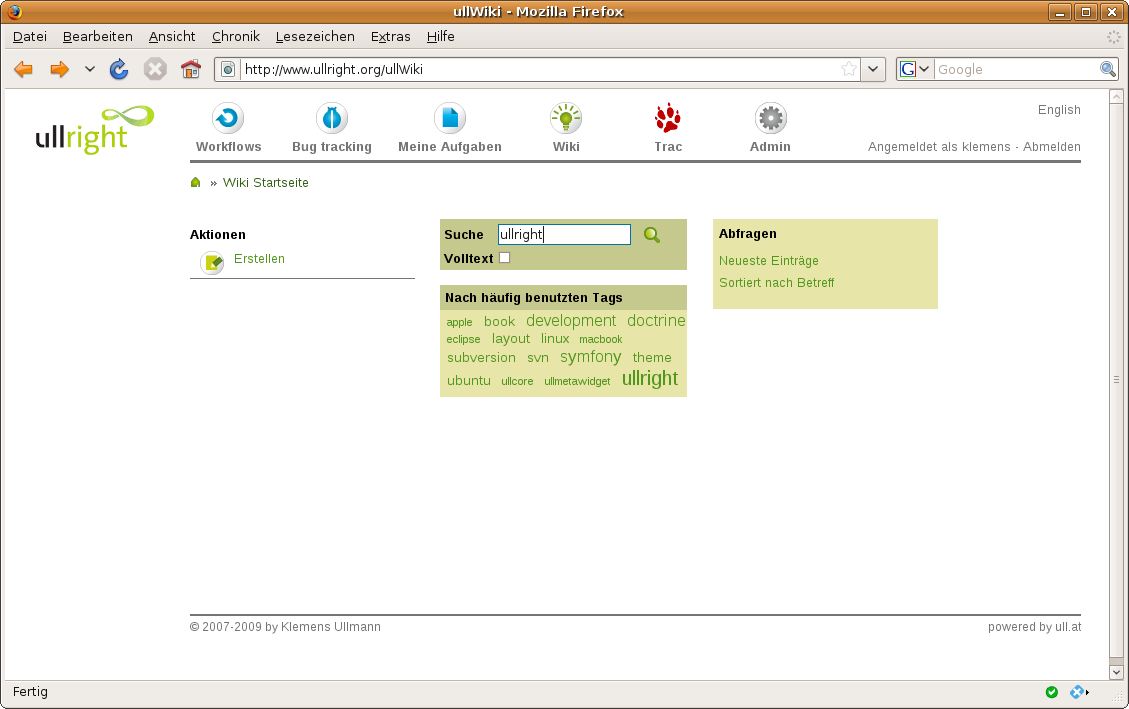
\includegraphics[width=0.9\textwidth]{index}
\caption{Startseite}
\label{fig:index}
\end{figure}

\subsection{Neues Dokument erstellen}
Häufig möchte man schnell einen Gedanken oder Einfall dokumentieren. Dafür ist natürlich der Punkt ein neues Dokument zu erstellen am wichtigsten. Falls Sie noch nicht in "`ullright"' angemeldet sind, werden sie praktischerweise sofort zur Anmeldemaske weitergeleitet. Auch nach der Anmeldung landen Sie nicht irgendwo, sondern direkt auf der Erstellungsseite.

\subsection{Suchfunktionen}
Geben Sie einfach jeglichen gewünschten Begriff in das Suchfeld ein. Wenn Sie auch den Text der Dokumente durchsuchen wollen, haken Sie bitte "`Volltext"' an. Die Suchfunktion sucht in den Feldern Id, Betreff und Tags.

Sie können Dokumente auch direkt anhand von Tags auswählen. Klicken Sie dazu einfach auf einen Tag und Sie erhalten eine Liste aller Dokumente für die dieses Tag vergeben wurde

\subsection{Abfragen}
Verwenden Sie die Abfragen um alle Einträge anzusehen. Individuelle Abfragen ergänzen wir Ihnen gerne auf Anfrage.



\section{Ergebnisliste}
Auf der Ergebnislisten-Maske haben Sie alle wichtigen Funktionen zur Verfügung (Siehe Abbildung \vref{fig:list}):

\begin{itemize}
\item Neues Dokument erstellen
\item Suche
\item Ergebnislisten
\end{itemize}
Aus diesem Grund verlinkt ullright standardmäßig auf die Ergebnisliste des Wikis, und nicht auf die Startseite.

\begin{figure}[htp]
\centering

\includegraphics[width=0.9\textwidth]{list}
\caption{Ergebnisliste}
\label{fig:list}
\end{figure}


\subsection{Anzahl der Ergebnisse und Blättern}
Sie sehen die Anzahl der gefunden Dokumente, und welche Einträge gerade angezeigt werden. Standardmäßig werden 30 Einträge pro Seite angezeigt. Benutzen Sie die Funktion "`Blättern"' auf der rechten Seite um zur nächsten, oder einer beliebigen Seite der Ergebnisliste zu kommen.

\subsection{Liste}
Damit Sie die neuesten Einträge stets in Griffweite haben, sortiert die Ergebnisliste standardmäßig nach dem Aktualisierungsdatum. Sie finden also die zuletzt geänderten Dokumente ganz oben.

Klicken Sie auf eine der Spaltenüberschriften um nach dieser Spalte zu sortieren. Klicken Sie ein weiteres Mal um die Sortierung umzukehren.

Mittels der ersten beiden Symbole jeder Zeile können Sie einen Eintrag bearbeiten oder löschen.

Durch Klick auf den Betreff gelangen Sie zur Ansicht des Dokuments.

\subsection{Tipp: Die Browser Adresszeile als Kommandozeile}
Alle ullright Module unterstützen aktiv das sogenannte "`Deep Linking"'. Das bedeutet, daß alle wichtigen Parameter, wie zum Beispiel ein Suchbegriff, in der Adressleiste angeführt sind.

Sie können also jederzeit eine ullright Adresse als Bookmark (Favorit) speichern oder einer Kollegin per E-Mail schicken.

Beispiel: \url{http://www.ullright.org/ullWiki/list/filter[search]/openoffice}

Zeigt die Ergebnisliste für den Suchbegriff "`openoffice"'




\section{Erstellen und Bearbeiten}
Auch die Bearbeitungsseite präsentiert sich einfach und aufgeräumt (Siehe Abbildung \vref{fig:create-edit}).

Geben Sie einfach Betreff, Text, Tags und Zugriffsrecht an und Speichern Sie.

\begin{figure}[htp]
\centering
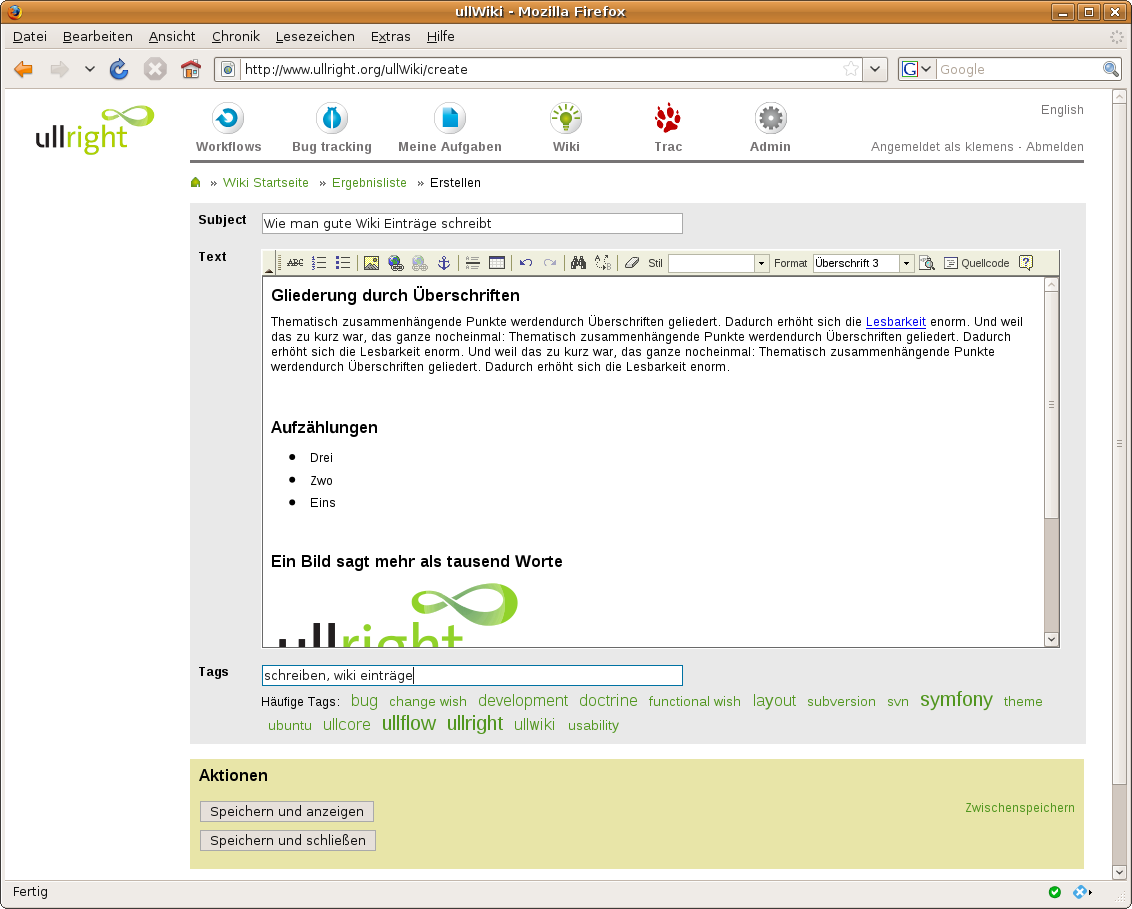
\includegraphics[width=0.9\textwidth]{create-edit}
\caption{Erstellen - Bearbeiten}
\label{fig:create-edit}
\end{figure}


\subsection{WYSIWYG Editor}
Viele Wikis verlangen nach HTML-Kenntnissen oder einer speziellen Syntax um den Text zu formatieren. ullWiki hingegen bietet einen komfortablen Editor, der ähnlich wie OpenOffice Writer oder MS Word funktioniert. Auch das Einfügen von Bildern oder Anhängen ist, wie weiter unten beschrieben, leicht möglich.

Bitte beachten Sie, dass die von uns ausgewählten Formatierungsmöglichkeiten nach semantischen Gesichtspunkten ausgewählt wurden. Sie finden also nur "`logische"' Auszeichnungen wie zum Beispiel "`wichtig"' oder "`Überschrift"', und keine rein optischen Formatierungsmöglichkeiten wie Farben oder Schriftgrößen. Somit werden saubere und zukunftssichere Teste gewährleistet. (Stichwort "`semantic Web"')

"`WYSISYG"' steht übrigens für "`What you see is what you get"', also sinnhaft man sieht schon beim bearbeiten genau wie es im Ansichtsmodus aussehen wird.

\subsection{Tags}
Vergeben Sie sinnvolle Tags um das Dokument zu kategorisieren und die Suche zu vereinfachen. Häufig benutzte Tags werden bereits angezeigt und müssen nur angeklickt werden.

\subsection{Zugriffsrecht}
Viele Wikis bieten komplizierte Zugriffsrechts-Mechanismen die oft umständlich zu bedienen sind. Häufig müssen Sie hierbei für jedes Dokument erneut auswählen welche Benutzer und Gruppen Zugriff darauf haben sollen.

Nicht so bei ullWiki: Wir stellen eine erweiterbare Liste an Zugriffsrechten zur Verfügung. Jedes Zugriffsrecht kann im Hintergrund komplexe Berechtigungen auf Benutzer und Gruppenebene enthalten.

Wählen Sie nun also einfach das gewünschte Zugriffsrecht für das aktuelle Dokument aus der Liste aus.

Standardmäßig finden Sie folgende Zugriffsrechte in der Liste:

\begin{itemize}
\item Öffentlich lesbar – Jeder kann lesen und angemeldete Benutzer können bearbeiten.
\item Für angemeldete Benutzer lesbar – Nur angemeldete Benutzer können lesen und bearbeiten.
\end{itemize}
Die Liste der Zugriffsrechte kann beliebig erweitert werden – Siehe Punkt "`Administration"'.

\subsection{Speichern}
Damit Sie möglichst effizient Arbeiten können, stellen wir mehrere Buttons zum Speichern zur Verfügung. So sparen Sie zum Beispiel bei "`Zwischenspeichern"' mehrere Klicks im Vergleich zu anderen Wikis, die nur einen "`Speichern"' Button bieten, und Sie zum weiter-bearbeiten erneut zur Bearbeitungsseite navigieren müssen.

\begin{itemize}
\item Speichern und anzeigen: Speichert das Dokument und zeigt die Ansichtsseite
\item Speichern und schließen: Speichert das Dokument und kehrt zurück zur Ergebnisliste
\item Zwischenspeichern: Speichert aber bleibt auf der Bearbeitungsseite
\end{itemize}

\subsection{Automatisches Speichern}
Während Sie ein Wiki-Dokument editieren speichert das System regelmäßig im Hintergrund Ihre Änderungen. Sie können nebenbei wie gewohnt arbeiten. Der Vorgang des Speicherns wird durch die Einblendung \emph{Automatisches Speichern ...} gekennzeichnet. Im Erfolgsfall erscheint \emph{Gespeichert}. 

Falls beim Automatischen Speichern ein Fehler auftritt wird eine entsprechende Meldung eingeblendet. Zusätzlich erscheint ein Button, der die Möglichkeit bietet, die Gründe für das Fehlschlagen des Speichervorgangs anzuzeigen.

\textbf{Achtung:} Das Automatische Speichern wird nur bei der Bearbeitung eines Wiki-Dokuments automatisch aktiviert. Falls Sie ein neues Dokument erstellen müssen Sie es erstmalig \emph{Zwischenspeichern} um das Automatische Speichern zu aktivieren. 




\section{WYSIWYG Editor im Detail}
Es folgen die Beschreibungen der wichtigsten erweiterten Funktionen.

\subsection{Bild einfügen}
(Siehe Abbildung \vref{fig:upload-picture})
\begin{itemize}
\item Setzten Sie den Cursor an die gewünschte Stelle im Text
\item Klicken Sie auf das Bildsymbol 
\includegraphics[width=5mm, height=5mm]{picture-symbol.png}
\item Wählen Sie "`Server durchsuchen"'
\item Wählen Sie ein Bild aus der Liste, oder laden Sie ein neues Bild hoch und wählen Sie es dann aus
\item Klicken Sie auf "`OK"'
\end{itemize}

\begin{figure}[htp]
\centering
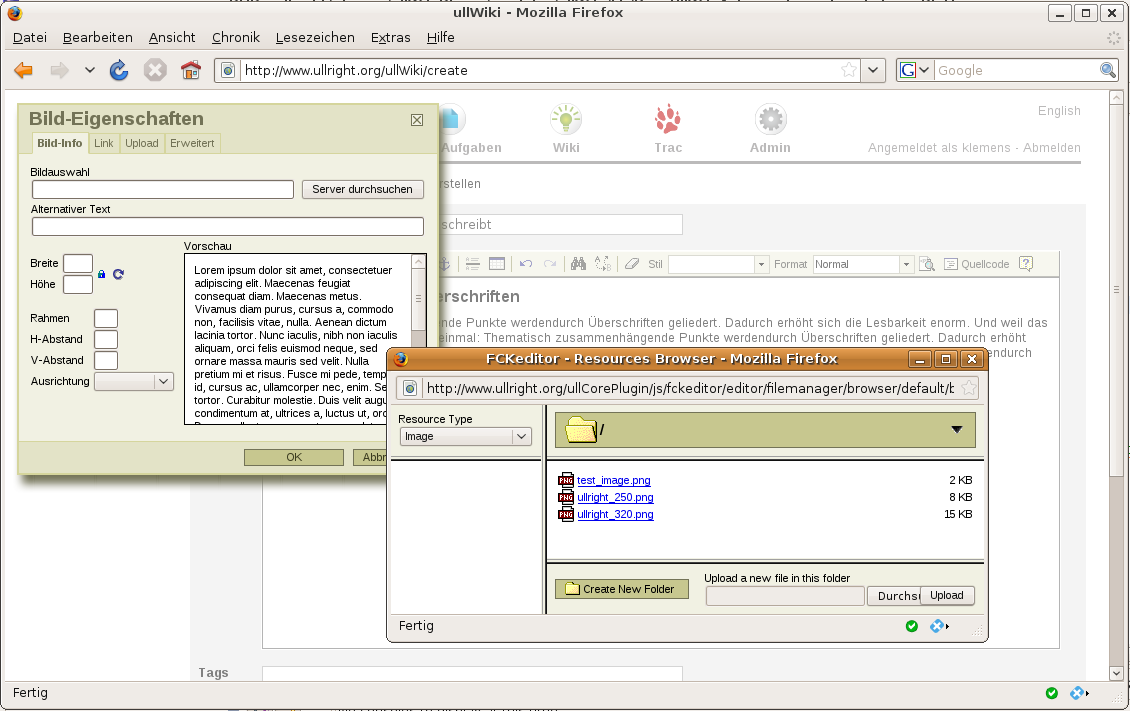
\includegraphics[width=0.9\textwidth]{upload-picture}
\caption{Bild hochladen}
\label{fig:upload-picture}
\end{figure}


\subsection{Link einfügen}
\begin{itemize}
\item Markieren Sie die Wörter im Text die Sie verlinken möchten
\item Klicken Sie auf das Linksymbol 
\includegraphics[width=5mm, height=5mm]{link-symbol.png}
\item Geben Sie die Adresse (URL) ein
\item Klicken Sie auf "`OK
\end{itemize}




\section{Ansicht}
Durch Klick auf den Betreff in der Ergebnisliste wird das Dokument im Ansichtsmodus geladen (Siehe Abbildung \vref{fig:show}).

Mittels der ersten beiden Symbole "`Stift"' und "`Mülleimer"' können Sie einen Eintrag bearbeiten oder löschen.

Am Ende des Dokuments erfahren Sie Detailinformationen zum Dokument, also wer und wann es erstellt hat, und wer und wann es aktualisiert hat.

\begin{figure}[htp]
\centering
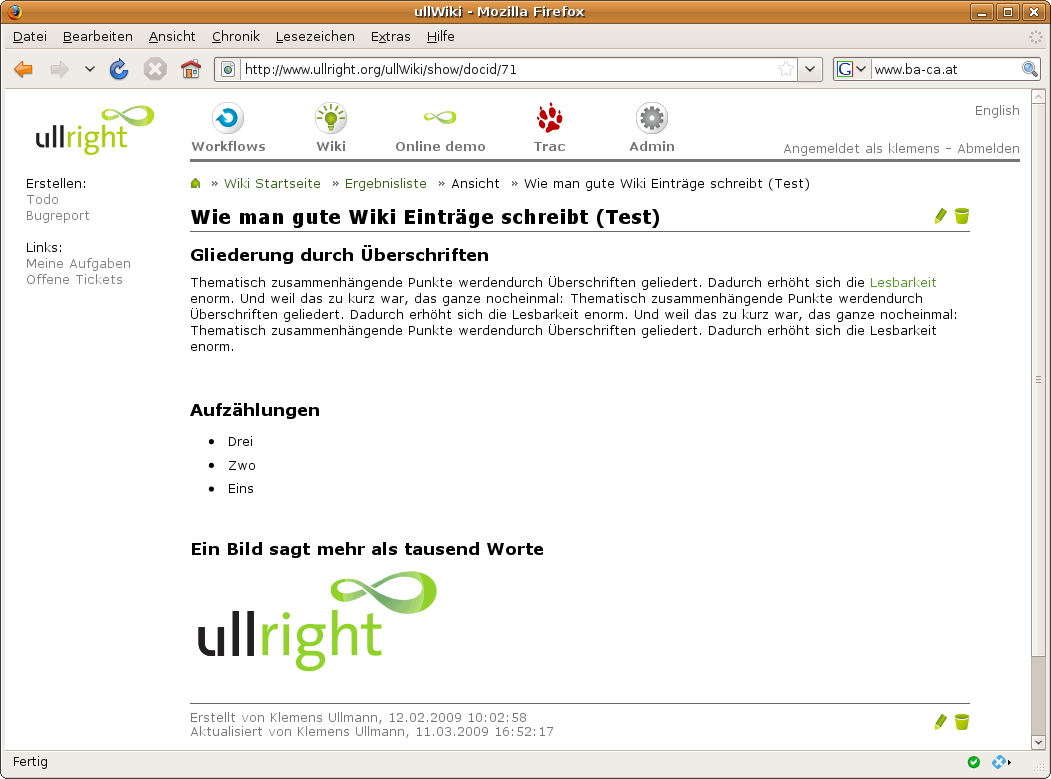
\includegraphics[width=0.9\textwidth]{show}
\caption{Ansicht eines Eintrags}
\label{fig:show}
\end{figure}




\section{Administration - Zugriffrechte}
Melden Sie sich als Benutzer mit Masteradmin-Rechten an und wählen Sie im Hauptmenü den Punkt "`Admin"'.

Blättern Sie hinunter bis zum Punkt "`Wiki"'.

\subsection{Anlegen}
Wenn Sie ein neues Zugriffsrecht anlegen möchten klicken Sie auf "`Verwalte Liste der Zugriffsrechte"' und erstellen Sie dort einen neuen Eintrag. Geben Sie eine eindeutige Bezeichnung (system-intern), sowie eine deutsche und englische Bezeichnung für das neue Zugriffsrecht ein.

\subsection{Zugriffsrecht konfigurieren}
Um für jedes Zugriffsrecht einzustellen wer was darf wählen Sie im "`Admin"' Bereich "`Wiki"' den Punkt "`Verwalte Zugriffsrechte"'.

Sie sehen nun eine Liste welche Gruppe welches Privileg (lesen, schreiben) pro Zugriffsrecht hat.

Erstellen Sie einfach neue Einträge nach Ihren Wünschen.

\subsection{Beispiel}
Zugriffsrecht für die Abteilung "`Einkauf"' erstellen. Nur Mitglieder der Abteilung Einkauf sollen die Einträge lesen und bearbeiten dürfen.

Falls die dafür erforderliche Benutzergruppe "`Einkauf"' noch nicht angelegt ist:
\begin{itemize}
 \item Admin $\rightarrow$ Verwalte Gruppen $\rightarrow$ Gruppe "`Einkauf"' anlegen
 \item Admin $\rightarrow$ Verwalte Gruppenmitgliedschaften $\rightarrow$ Die Mitarbeiter der Abteilung Einkauf zur Gruppe "`Einkauf"' hinzufügen
\end{itemize}

Nun wird das Wiki-Zugriffsrecht erstellt:
\begin{itemize}
 \item Admin $\rightarrow$ Sektion "`Wiki"' $\rightarrow$ Verwalte Liste der Zugriffsrechte $\rightarrow$ Neues Zugriffsrecht "`Einkauf"' anlegen
\end{itemize}

Und zuletzt wird das Zugriffsrecht konfiguriert:
\begin{itemize}
 \item Admin $\rightarrow$ Sektion "`Wiki"' $\rightarrow$ Verwalte Zugriffsrechte
 \begin{itemize}
  \item Erstellen $\rightarrow$ 
  \begin{itemize}
   \item Gruppe: Einkauf
   \item Privileg: Lesen
   \item Zugriffsrecht: Einkauf
   \item Speichern!
  \end{itemize}
  \item Erstellen $\rightarrow$ 
  \begin{itemize}
   \item Gruppe: Einkauf
   \item Privileg: Schreiben
   \item Zugriffsrecht: Einkauf
   \item Speichern!
  \end{itemize}
 \end{itemize}
\end{itemize}


\end{document}
